\chapter{Stato dell'arte} %\label{1cap:spinta_laterale}
% [titolo ridotto se non ci dovesse stare] {titolo completo}
%

\section{Background}
Al giorno d'oggi è sempre più frequente adottare soluzioni che facciano uso di moduli intelligenti all'interno dei più svariati ambiti lavorativi, ed è oramai risaputo come tali soluzioni, debbano rispettare tutta una serie di standard qualitativi, affinché possano essere ritenuti attendibili ai loro scopi. Tuttavia recenti studi hanno dimostrato un nuova gamma di difetti che evidenziano una serie di vulnerabilità, fin ora non riscontrate all'interno dello sviluppo software (tra cui, come verrà approfondito in seguito in questo capitolo, quelle dovute alla la Software Fairness), legati all'operare in maniera imparziale ed equa nel loro contesto di utilizzo \cite{brun2018software}.\\

Per capire come il mondo dello sviluppo software (ed in particolare quello delle soluzioni "intelligenti"), siano influenzati dagli aspetti di equità o un qualsiasi altro aspetto qualitativo in generale è doveroso introdurre gli aspetti essenziali che si pongono alla base dello sviluppo di tali applicativi.\\\\

\subsection{Ingegneria del Software}
Prima di tutto è senz'altro necessario far riferimento all'Ingegneria del Software, disciplina che nasce proprio in risposta alle problematiche di sviluppo di prodotti software di qualità in un preciso tempo, con uno specifico budget \cite{Bruegge2009ObjectOrientedSE}. L'ingegneria del Software si pone l'obiettivo di applicare tutta una serie di attività che facciano dello sviluppo software un vero e proprio processo ingegneristico \cite{mall2018fundamentals}. Le attività cardine dell'Ingegneria del Software sono \cite{Bruegge2009ObjectOrientedSE}:

\begin{itemize}
    \item La \textbf{modellazione}: capacità standard di focalizzarsi sui dettagli rilevanti ignorando tutto il resto, tramite svariate strategie di raffinamento e astrazione;
    \item Il \textbf{problem solving}: l'utilizzo di modelli per la ricerca di soluzioni a specifici problemi;
    \item L' \textbf{acquisizione di conoscenza}: la raccolta di singoli dati e informazioni di uno specifico dominio, per poi formularne informazioni e conoscenza prima di applicare standard di sviluppo;
    \item La \textbf{ricerca di un razionale}: cioè la ricerca delle motivazioni e delle necessità che si pongono a priori dello sviluppo di un tool software;
\end{itemize}

Si osserva quindi come effettivamente un tool software per essere progettato in maniera congrua a molteplici aspetti qualitativi -ad esempio: sicurezza, manutenibilità e adattabilità (o qual si voglia tipologia di attributo non funzionale) - che soddisfino le aspettative del cliente che lo commissiona, sia necessario applicare un processo standard di ingegnerizzazione. Nello specifico, anche problematiche legate all' emergente tematica dell'equità e dei vincoli di imparzialità devono essere trattati sullo stesso piano di un qualsiasi altro attributo qualitativo e la ricerca si sta muovendo sempre di più in questa direzione \cite{brun2018software}.
    

\subsection{Intelligenza Artificiale e Machine Learining}
L'Intelligenza Artificiale ed in particolare i moduli di Machine Learning, stanno diventando sempre di più una parte fondamentale delle applicazioni commerciali e dei progetti di ricerca nell'ambito IT. In particolare si osserva come i moduli addestrati delle applicazioni di maggior successo, siano realizzate a partire dalla generalizzazione di esempi noti (basi di conoscenza), sulle quali i moduli stessi vengono addestrati, al fine di produrre, sulla base di dati di input forniti, un output desiderato senza che l'utente umano dia informazioni aggiuntive. La branca del Machine Learning, nella quale vengono racchiusi tutti glia algoritmi che si basano su tali tuple di \textit{input-output} viene definita come  \textbf{Apprendimento Supervisionato} \cite{libroMLs}.

Dalla stessa fonte possiamo osservare come esempi di apprendimento supervisionato di interesse possano essere:
\begin{itemize}
    \item L'identificazione di \textit{topix} da un blog o un sito internet;
    \item l'identificazione di pattern di accesso anomali in un sito web;
    \item la suddivisione dei clienti di uno shop per preferenze similari.
\end{itemize}

\begin{comment}
\begin{figure}[htpb]
    \centering
    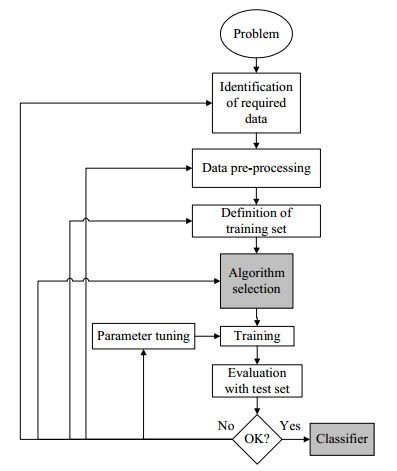
\includegraphics[width=\textwidth,height=10cm,keepaspectratio=true]{supervisedML}
    \caption{
        Processo standard di un algoritmo di Machine Learning Supervisionato dall'articolo \cite{supervisedML&Classification}
    }
    \label{fig:basics AFM sketch}
\end{figure}%
\end{comment}

Soprattutto negli ultimi anni, si ci sta accorgendo che l'applicazione combinata di discipline come la statistica, la teoria dell'informazione e il machine learning, stanno portando alla creazione di una scienza sempre più solida, con una ferma base matematica, e a tool sempre più potenti. In particolare, se si fa riferimento al learning supervisionato tecniche e algoritmi come alberi di decisione, regressione lineare, regressione logistica, clustering, sono alcune delle tecniche più utilizzate per la progettazione di componenti AI, per innumerevoli campi applicativi, ed In particolare quello che ne risulta dall'applicazione di una generica tecnica di learning supervisionato, su un dataset di addestramento, è definito come processo di Classificazione \cite{supervisedML&Classification}. \\

Per capire praticamente la problematica di classificazione in ambito machine learing, si può pensare di far riferimento al comune esempio di identificazione delle mail di spam. Oramai numerosi gestori di mailing utilizzano tecniche automatiche di filtering per le mail di spam, sulla base di grandi data set a disposizione del tool. In pratica, sulla base dei dati (strutturali, storici e similari) a disposizione di mail già contrassegnate o meno come "Spam Mail" è possibile addestrare un modello, al fine di classificare una nuova mail che un generico utente riceve come "SPAM MAIL" oppure "NON SPAM MAIL". Volendo dare quindi una definizione semi formale: il problema di classificazione del Machine Learning consiste nell'\textit{individuare una \textbf{categoria} (ad esempio MAIL di SPAM oppure MAIL NON DI SPAM) per una \textbf{nuova osservazione} (e.g. una nuova mail ricevuta), sulla base di precedenti \textbf{dati di addestramento}contenenti informazioni già classificati secondo \textbf{categorie note} (ad esempio archivio di mail già classificate come SPAM oppure NON SPAM a disposizione del modulo addestrato}"\cite{FairnessDefinitionExplained}.\\

Questa problematica è particolarmente attenzionata dalla ricerca, dato che è molto complesso generare classificatori che non soffrano di alcuni problemi noti in letteratura, come ad esempio, la stretta dipendenza dal Data Set di partenza \cite{supervisedML&Classification}, il così detto fenomeno del \textit{garbage-in,garbage-out}, cioè la presenza di Bias nei dataset di addestramento, che poi tenderanno a riflettersi all'interno delle predizione dei moduli di previsione stessi\cite{evalFairClassification}.\\

\cite{evalFairClassification} Volendo porre un esempio pratico, nell'ambito dell'etica del software, è facile che un classificatore addestrato con un dataset, non immune a dei bias su specifici attributi sensibili (quali razza o sesso), possa essere addestrato in modo tale da effettuare predizioni imparziali, spesso rivolte a favore degli individui del campione di addestramento dei gruppi di maggioranza (ovvero quegli individui che posseggono il valore più ricorrente dell'attributo sensibile).


\subsubsection{Algoritmi di ricerca e Algoritmi Genetici}
Il machine learnig è sicuramente uno degli aspetti più caratterizzanti dell'intelligenza artificiale, al fine di fornirne una panoramica più ampia è interessare considerare anche gli algoritmi di ricerca. Essi per definizione sono usati per restituire informazioni memorizzate all'interno di strutture dati o ricercare soluzioni in un complesso spazio di ricerca formalmente definito sulla base del dominio del problema, il tipo di informazioni gestite dagli algoritmi di ricerca possono essere formate da valori discreti e continui. Di algoritmi di ricerca ne esistono in letteratura di vari tipi, basati su vari approcci: Algoritmi basati sull'uso di una funzione di costo (e.g. depth-first, bread-first e cost-uniform first...), basati sull'utilizzo di euristiche (e.g. A* greedy best-first), algoritmi di ricerca locale (e.g. hill-climbing search) ecc., ma tra i più usati in ambito di ricerca ci sono sicuramente gli algoritmi di tipo evolutivo ed in particolare quelli di tipo genetico.

\cite{geneticalgotihm}Gli algoritmi genetici, sono algoritmi di ricerca basati sui principi della selezione naturale e della genetica, introdotti negli anni '70  da J.Holland e ispriati alle teorie dell'evoluzione degli esseri viventi. Gli algoritmi genetici astraggono lo spazio del problema come una popolazione di individui, e provano ad esplorare le caratteristiche degli individui, "producendone" di nuovi in maniera iterativa. I GA evolovono la popolazione da individui iniziali (spesso generati casualmente) in individui di alta qualità, laddove ogni individuo rappresenta una soluzione al problema di interesse codificata in stringa. La qualità di ogni individuo è misurata da una funzione matematica detta funzione di fitness che è formulata in modo tale da valutare in maniera quantitativa la bontà di un individuo, a seconda di alcune caratteristiche qualitative definite dallo sviluppatore. - A seconda del problema la funzione di fitness, può essere di massimizzazione, di minimizzazione, a singolo obiettivo o multi obiettivo, e spesso rappresenta l'ostacolo più grande nella progettazione di un algoritmo genetico. - \\

\cite{geneticalgotihm} Durante ogni generazione, tre operatori di base della genetica sono applicati in sequenza con una certa probabilità: selezione, crossover e mutazione. I passaggi base di un algoritmo di ricerca genetrico sono:
\begin{enumerate}
    \item Generazione randomica di una popolazione di n individui (rappresentanti di soluzioni randomiche al problema);
    \item Valutazione di ogni individui tramite la funzione di fitness;
    \item Selezione di due individui per generarne di nuovi (nuova generazione), le tecniche di selezione possono essere diverse, tra le più famose ci sono: la roulette wheel e l'approccio a torneo;
    \item Con una certa probabilità, viene applicata un operazione di cross over al fine di mischiare singole parti degli individui selezionati per generarne di nuovi (anche qui ne esistono vari tipi). se il crossover non viene applicato, in sostituzione vengono copiati "i genitori";
    \item Con una certa  probabilità ai nuovi individui vengono applicate operazioni di mutazione (ovvero vengono cambiati uno o più dati della stringa casualmente);
    \item Gli individui generati, vengono aggiunti alla popolazione, al fine di far ripartire l'algoritmo;
    \item Se uno degli individui generati soddisfa le condizioni di accettazione e di arresto dell'algoritmo, allora si ritorna la soluzione migliore trovata fino a quel momento;
    \item Altrimenti l'algoritmo riparte dal passo 2;
    
\end{enumerate}


\subsection{Ingegneria del Software nell'Intelligenza artificiale}

Si può osservare come negli ultimi decenni, l'intelligenza artificiale e l'ingegneria del software, si siano evolute separatamente. Oggi giorno, si osserva però come la ricerca attuale, stia portando alla specifica e alla costituzione di nuovi studi e approcci allo sviluppo di soluzioni AI-Intensive, che tengano proprio conto dell'intersezione che c'è tra l'ingegneria del software e l'intelligenza artificiale \cite{rech2004artificial}. \\

Prima di entrare nel dettaglio di quest'intersezione è necessario capire perché, le soluzioni AI-Intensive, necessitano di essere progettate e sviluppate con approccio ingegneristico, così come stabilito nell'articolo \textit{Artificial Intelligence \& Ethics} publicato sull'Harvard Magazine nel 2019, l'Intelligenza artificiale, oggi giorno, fa riferimento a sistemi che sulla base degli input che ricevono in considerazione devono assumere rischi, fare predizioni o assumere comportamenti in risposta a specifici problemi \cite{shaw2019artificial}. In dettaglio, nell'era dei computer dalle elevate prestazioni e dei Big Data, molte soluzioni AI-Intensive, sono sviluppate in risposta ai bisogni che la quotidianità sociale necessita, ma come noto in letteratura, molti sistemi software di grandi dimensioni, non sono privi di Bug, ed in particolare i sistemi basati sull'AI e il Machine Learning non fanno eccezione. In dettaglio, questa tipologia di sistemi, dei bug di progettazione o addestramento, possono portare a crush di sistema, output errati fino all'esecuzione troppo lenta che non rende possibile l'utilizzo di tali soluzioni nell'ambiente di lavoro \cite{ML&Bugs}. In casi critici gli errori dei sistemi intelligenti, possono addirittura portare alla morte di chi anche involontariamente interagisce con essi, il caso più noto è quello della ciclista Elaine Herzberg, morta investita da un'auto con pilota automatico, per errore di valutazione del modulo di guida \cite{shaw2019artificial}. Quindi come è possibile produrre soluzioni AI Intensive per il mondo reale, che tengano conto di tali problematiche? L'applicazione dell'ingegneria del software cerca in qualche modo di dare risposta a questa tipologia di problematica.\\


In dettaglio, L'Ingegneria del software, include metodi di Requirement Engineering, Design Engineering, Code Engineering e Project Management, che possono essere di supporto, per lo sviluppo di Sistemi Ai-Intensive efficienti. La ricerca stessa ne fa utilizzo, ed infatti molti ambiti di studio sono nati dall'intersezione tra SE e AI, in particolare l'Agent Oriented Software Engineering oppure l'Ambient Intelligence \cite{jain2011interaction}.\\

L'Agent Oriented Software Engineering, si concentra sullo sviluppo di soluzioni che siano, intelligenti, agili e pro-attive. In dettaglio il suo scopo principale è quello di sviluppare soluzioni AI-intensive tramite dei riadattamenti stessi delle tecniche di Ingegneria del Software, per lo sviluppo di Agenti di piccoli e grandi dimensioni. Nel dettaglio risultano essere di rilievo l' \textit{Agent UML}, per la progettazione dei moduli agente, oppure metodi di specifica e valutazione formali dei sistemi, i quali hanno lo scopo intrinseco di validare gli obiettivi, i comportamenti di un singolo agente, e soprattutto le interazioni nei sistemi multi agente \cite{rech2004artificial}.l'Ambient Intelligence invece si pone lo scopo di progettare ambienti di addestramento (secondo tecniche specifiche dell'ingegneria del software) che siano sensibili ed adattabili agli stimoli esterni e in conseguenza, sistemi reattivi che siano informati circa i bisogni, le abitudini e le emozioni degli utenti per supportare il loro lavoro quoridiano\cite{rech2004artificial}.\\

Qualsiasi branca o studio di ricerca a cui si voglia far riferimento (come gli esempi riportati) definita "intersezione tra intelligenza artificiale e ingegneria del software", non può prescindere dall'analizzare quelli che sono i requisiti non funzionali di qualità che una soluzione AI-Intensive deve rispettare. In particolare in letteratura \cite{NFRForML}, si può osservare come, ad esempio, il Machine Learning sia soggetto a specifici vincoli di qualità quali: 

\begin{itemize}
    \item \textbf{Accuracy and Performances}, come l'output di un agente risulta "corretto" se paragonato alla realtà;
    \item \textbf{Fairness}, Requisito che si pone l'obiettivo di rendere gli algoritmi di ML più \textbf{imparziali} e indipendenti da bias di dati;
    \item \textbf{Transparency}, ovvero la capacità di dimostrare come i risultati elaborati da un modulo intelligente siano affidabili e trasparenti, ricostruendo le fonti di partenza;
    \item \textbf{Security and Privacy}, \textbf{Testability} e \textbf{Reliability} del modulo addestrato.
\end{itemize}

Per progettare, realizzare e controllare questi aspetti qualitativi essenziali per un modulo di intelligenza artificiale, la ricerca è enoremente incentrata nello studio di questi aspetti. In particolare, si nota come questi Requisiti Non Funzionali, siano particolarmete attenzionati dall'ingegneria dei requisiti, branca dell'ingegneria del software che si incentra nella specifica, l'analisi, la verifica e la validazione dei requisiti di un sistema software \cite{RE&Ai}, la cui ricerca ricerca sta incentrando buona parte dell'effort nello studio di aspetti quali fairness, privacy, sostenibilità e modificabilità anche per tecniche di Machine Learning e per lo sviluppo di soluzioni AI-Intensive in generale \cite{NFRForML}.

\cite{RE&Ai}In particolare, la letteratura afferma come l'indistria dell'intelligenza artificiale è particolaremente incentrata nello sviluppo di soluzioni di Machine Learning e basate sugli approcci Data Driven, ed una delle principali aree di interesse per lo sviluppo di questo tipo di soluzion è il settore dell'Healtcare, particolarmente caratterizzato dalla mancanza di standard di progettazione e dalla continua evoluzione dei dati a disposizione. Per far fronte a questa tipologia di problematiche, l'ingegneria del software ed in particolare l'ingegneria dei requisiti, pone l'accento su nuove metodologie e tecniche che toccano vari processi di un sistema AI-Intensive: la specifica e l'analisi dei suoi requisiti, la validazione del modello (e quindi delle sue specifiche), la documentazione e il management dell'intero processo di sviluppo dei requisiti formulati. Le sfide principali che la ricerca ha davanti in quella che è stata definita \textit{intersezione} tra intelligenza artificiale e ingegneria del software sono:

\begin{itemize}
    \item \textbf{Lo Skill Gap}: la necessità di creare lo giusto spirito di collaborazione aziendale tra Data Scientists e Ingegneri del Software;
    \item \textbf{Il Data Gap}: Ovvero la necessità di rendere disponibili (big) dataset necessari alla realizzazione di soluzioni AI complesse;
    \item \textbf{Engeeniring Gap}, ovvero la necessità di creare prototipi generalizzabili dei sistemi AI, con il giusto supporto all'intero ciclo di vita della Soluzione AI-Intensive;
\end{itemize}

\subsection{Software Fairness}
Dopo aver introdotto il macro ambito in cui l'elaborato si colloca, è senz'altro necessario introdurre quello che è l'aspetto principale che caratterizzerà il lavoro illustrato nei successivi capitoli, ovvero la Software Fairness e il codice eticalmente corretto. Come già introdotto nel precedente paragrafo, l'articolo \textbf{Non-Functional Requirements for Machine Learning: Challenges and New Directions} \cite{NFRForML}, introduce alla fairness come un requisito non funzionale dei moduli di machine learning, per il quale  le attività di ricerca attuale sta investendo molto. In particolare si cerca di rendere gli algoritmi di machine learning più imparziali, non solo cercando di rimuovere features sensibili (come razza o sesso), ma cercando soprattutto di definire e implementare soluzioni AI-Intensive che tengano conto del livello di fairness richiesto dal dominio di applicazione.\\

\cite{NFRForML} Implementare un algoritmo eticalmente corretto, significa definire formalmente cosa si intende per fairness, e cercare in conseguenza di misurare come ciò  viene implementato, \cite{evalFairClassification} ma fare questo non è così immediato. Dato che  concetto di Fairness è relativamente nuovo per la comunità scentifica, e soprattutto requisiti sociali e principi legali spesso ne evidenziano differenti caratteristiche,  sono emerse differenti definizioni del concetto e un numero speculare di metriche per misurarne il livello nei sistemi software.

Prima di cercare di definire formalmente il concetto però è necessario cercare di capire in che maniera un sistema software mostra dei comportamenti scorretti e nello specifico , e come la comunità scientifica si pone rispetto ad esso.   

\cite{brun2018software} Recenti studi, inerenti gli aspetti di qualità e il successo del Processo Ingegneristico del software, hanno dimostrato che i sistemi software presentano un nuovo tipo di vulnerabilità, correlate appunti alla loro abilità di operare in maniera imparziale (fair) e priva di pregiudizi. Da dove nasce, quindi il problema della software fairness? \cite{brun2018software} come espresso in letteratura, il livello di fairness è strettamente correlato al concetto di Bias (pregiudizi algoritmici) che un sistema software ha al suo interno, questi comportamenti erronei possono emergere da vari aspetti, soprattutto appresi dai dati di addestramento (per quanto concerne le soluzioni AI-Intensive), ma anche per specifiche di requisiti incomplete, design povero, bug di implementazioni o interazioni errate tra componenti. Esistono differenti esempi interessanti di come Bias nei sistemi software abbiano portato a spiacevoli inconvenienti, tra i più famosi vale la pena citare:

\begin{itemize}
    \item \textbf{Software di Recruiting}: \cite{amazonrecruiting2018reuters} Gli specialisti di Machine Learning di Amazon, hanno reso noto che nel 2015, il loro nuovo tool di recruiting per lo sviluppo o altre posizioni tecniche, non offriva opportunità lavorative in maniera imparziale rispetto al sesso dei candidati, questo perchè tale sistema era addestrato con dei dati di un periodi di 10 anni antecedente al 2015, per il quale la prevalenza degli impiegati tecnici dell'azienda è stata maschile, il gender e altri fattori (quali razza, oppure lo stesso linguaggio che gli impiegati tecnici maschili hanno adottato negli anni), sono stati classificati come feature sensibili che hanno addirittura portato Amazon, a chiudere il progetto, secondo quanto stabilito dalla loro versione ufficiale;
    
    
    \item \textbf{Healt Care}: \cite{HealtCareBias} Gli ospedali statunitensi per anni hanno utilizzato un software di predizione, per le cure mediche, che nel tempo è arrivato a "preferire" i pazienti di razza bianca, rispetto a quelli di colore. Tale comportamento "unfair" è da attribuire, purtroppo ad un bias di dati che considerava più "conveniente" la popolazione bianca, dato che quest'ultima era soggetta a spese mediche maggiori rispetto a quelle di colore, quindi "secondo il tool" preferendo tali individui su un campione di più di 200 milioni di abitanti, ci sarebbero stati maggiori guadagni per gli ospedali pubblici americani. Tale assunzione però si è convertita nella pratica nel considerare le persone di colore, maggiormente in salute rispetto quelle di carnagione chiara;
    
    \item \textbf{Crimine}: \cite{biasblack2016propublica} Nel 2014, si è osservato come un tool  (denominato Correctional Offender Management Profiling for Alternative Sanctions, meglio conosciuto con l'acronimo di COMPAS), di predizione di responsabili di futuri crimini tra i più usati in Florida tra il 203 e il 2014, il cui funzionamento si basa sul confronto di analisi facciali partendo da  un dataset di immagini di fotografie di criminali condannati, avesse la tendenza a giudicare le persone di colore come più più predisposte a crimini violenti quali, la causa di questa tematica è ancora oggi molto discussa, ma si ritiene che la causa principale, sia nuovamente nei dati con cui il modello veniva addestrato, nel quale erano presenti feature sensibili, quali razza o sesso;
    
    \item \textbf{Traduzioni Automatiche}: \cite{biasInML}, Si è risontrato come Google Traduttore, il più popolare motore di traduzione al mondo, mostrava un bias legato al sesso. in particolare, se si traduce dall'inglese al turco la frase "She is an engineer, He is a nurse", ne risulta un inversinone di sogetti: “He is an engineer, She is a nurse”, quasi ad indicare come le professioni tecniche, come un generico Ingegnere, in Turchia sia automaticamente associato al sesso maschile.
    
    \item \textbf{Generazione automatica di sottotitoli}: \cite{tatman-2017-gender} Su Youtube, se si seleziona la traduzione automatica, si osserva come effettivamente la traduzione del video risulti essere maggiormente accurata con voce maschile, rispetto a voce femminile, inoltre si osserva come che per lingue come l'inglese o l'arabo, ci siano delle differenze qualitative circa il risultato della traduzione, per alcuni specifici dialetti.
    

\end{itemize}

Dagli esempi osservati, si osserva quindi, come ricercatori e ingegneri del software producano sempre di più software di qualità, in risposta alla necessità di prendere delle decisioni eticamente corrette, che riguardano sempre di più la vita umana\cite{biasInML}. Di conseguenza, si nota come un tool software o una soluzione AI-Intensive utilizzata su larga scala, non possa più presentare vulnerabilità che vadano ad inficiare il suo livello di Fairness. In risposta a questa nuova issiue ingegneristica, ne deriva in maniera naturale che è necessario come applicare definire formalmente il concetto di Software Fairness e conseguenti processi standard di misurazione.\\\\


\cite{FairnessDefinitionExplained} Negli ultimi anni questa problematica, ha attirato l'attenzione di ricercatori nell'ambito dell'intelligenza artificiale, l'Ingegneria del software e la comunità legislativa, con più di venti differenti notazioni di Software Fairness proposte e ,ovviamente, quello che ne deriva è che non è che non è possibile darne un'unica definizione specifica, ma è necessario specializzare il concetto in riferimento ad una specifica problematica analizzata.\\

 Ponendo l'attenzione al problema di Classificazione del Machine Learning, già definito nel precedente paragrafo di introduzione all'intelligenza artificiale, è possibile dare numerose definizioni di Fairness per un generico classificatore ML, sulla base di alcuni strumenti ampliamente utilizzati nell'ambito dell'Intelligenza Artificiale, ovvero: Le misure statistiche di validazione, le misure di similarità e distanza e il Casual Reasoning. \cite{FairnessDefinitionExplained}.
 
 \subsubsection{Definizioni di Fairness basate su Metriche Statistiche}
 
 Il paper, \textbf{Fairness Definition Explained}, a cura dei ricercatori Sahil Verma e Julia Rubin \cite{FairnessDefinitionExplained}, introduce a questa tipologia di definizioni basate su metriche statistiche fornendo alcuni concetti di base: 
 
 \begin{itemize}
     \item Attributi sensibili o protetti: attributo di un dato dataset, sul quale si sta effettuando classificazione, per il quale il generico modulo AI di classificazione potrebbe produrre discriminazioni (come ad esempio Gender o razza);
     \item Diretta conseguenza degli attributi sensibili possono essere i Gruppi Protetti, gruppi di individui che assumono un valore dell'attributo sensibile che potrebbe essere soggetto a discriminazione;
     \item Il valore reale di classificazione: ovvero il valore (categoria di appartenenza) assegnato un individuo del dataset assume sulla base base delle sue feature di riferimento;
     \item La probabilità di predizione [0-1]: ovvero la probabilità condizionata che un individuo appartenga ad una data categoria, sulla base dei dati che lo caratterizzano, i classificatori, per stimare queste probabilità fanno riferimento in generale a tutte le feature del dataset, e in casi particolari possono anche riferirsi ad attributi sensibili, per particolari scelte di implementazione;
     \item La decisione predetta [0-1]: ovvero la categoria di appartenenza dell'individuo determinata dal classificatore, sulla base del dataset.
 \end{itemize}
 
 Le metodologie statistiche di validazione di un classificatore, ed in particolare i classificatori binari (con due singole categorie di classificazione, per convenzione una positiva e una negativa), fanno utilizzo di questi concetti, un determinato individuo può risultare:
 
 \begin{itemize}
     \item \textbf{Reale Positivo - True Positive} (TP), se il valore reale di predizione e la decisione predetta dal corrispondono entrambi alla categoria "positiva";
     \item \textbf{Reale Negativo - True Negative} (TN), se il valore reale di predizione e la decisione predetta corrispondono entrambi alla categoria "negativa";
     \item \textbf{Falso Positivo - False Positive} (FP), se la decisione predetta corrisponde alla categoria "positiva", mentre il valore reale di predizione è la categoria "negativa";
    \item \textbf{Falso Negativo - False Negative} (FN, se la decisione predetta corrisponde alla categoria "negativa", mentre il valore reale di predizione è la categoria "positiva".
 \end{itemize}, 
 
 Determinando questi valori per ciascuno degli individui del dataset, è possibile estrarre numerose metriche utili alla validazione di un generico classificatore binario, le più famose sono note in letteratura sono:
 
 \ldots la precision:
\begin{equation*}
\frac{\sum{TP}}{\sum{TP + FP}}
\end{equation*}


 \ldots  e la recall:
\begin{equation*}
\frac{\sum{TP}}{\sum{TP + FN}}
\end{equation*}

Tali formule, con altre metriche statistiche ampliamente riconosciute, sono spiegate nel dettaglio, nel paper  di riferimento\cite{FairnessDefinitionExplained}, vale la pena osservare che tali metriche possono essere generalizzate anche nel caso si stia validando un classificatore con N categorie.

Questa piccola introduzione ai concetti basilari di classificazione, permette quindi di introdurre a qualche definizione di Fairness tra le più utilizzate nell'ambito della classificazione, tra le più importanti e utilizzate, vale la pena citare (N.B. Le definizioni riportate prendono come dominio di applicazione i classificatori binari, così come gli attributi sensibili con due possibili valori)\cite{FairnessDefinitionExplained}:

 
\begin{enumerate}
     \item \textbf{Group Fairness - Statistical Parity}: Un classificatore, soddisfa questa definizione di fairness, se individui di un gruppo protetto (G1), definito per un dato attributo sensibile (g), possano essere assegnati dal classificatore alla categoria positiva ( che quindi il valore predetto d sia pari ad 1) , con la stessa probabilità degli individui del gruppo non protetto (G2), per il quale l'attributo sensibile assume valore non discriminante: P(d = 1| g = X1) = P(d = 1 | g = X2), dove X1 e X2 sono rispettivamente il valore discriminate e non discriminate dell'attributo sensibile g;
    
     \item \textbf{Predictive Parity - Outcome Test}: Un classificatore soddisfa questa definizione, se entrambi i gruppi, protetto e non protetto, hanno stessa probabilità di assumere valore reale di classificazione (Y), pari ad 1 (categoria positiva), data decisione predetta pari ad 1: P(Y = 1| d = 1 \& g = X1) = P( Y = 1 | d = 1 \& g = X2);
    
     \item \textbf{False Positive Error Rate Balance}: Un classificatore soddisfa questa definizione, se, la probabilità di essere classificati come appartenenti alla categoria positiva, (decisione predetetta d = 1), pur appartenendo in realtà alla categoria negativa (valore reale di classificazione Y = 1), sia equivalente sia per individui appartenenti al gruppo protetto che per quelli appartenenti al gruppo non protetto: P(d = 1| Y = 0 \& g = X1) = P( d = 1 | Y = 0 \& g = X2);
\end{enumerate}

Queste ed altre definizioni statistiche del concetto di Software Fairness, vengono illustrate più in dettaglio nel paper di riferimento \cite{evalFairClassification}, anche in termini di metriche di validazione statistica quali Precision e Recall. Quello che però è importante sottolineare è l'enorme dinamicità di queste definizioni statistiche, come  si nota come gli esempi riportati (come altre definizioni statistiche di Fairness presenti in letteratura), modellano concetti di probabilità differenti, ognuno avente un significato semantico ben preciso, e per avere una buona idea del livello statistico di Fairness di un classificatore sotto analisi, è necessario identificare bene quali metriche tenere in considerazione. Come è buona pratica di questi studi statistici può essere anche opportuno considerare e incrociare i risultati più metriche per formalizzare considerazioni più attendibili.

 \subsubsection{Definizioni di Fairness basate su Metriche di Similarità}
 
 Continuando questo excursus, nell'analisi delle definizioni di Software Fairness, nell'ambito dei classificatori ML, è possibile è possibile notare, come le definizioni statistiche, ignorino largamente tutti gli attributi di classificazione di un soggetto (sia X l'insieme degli attributi non sensibili di un generico individuo per cui si vuole effettuare classificazione), a meno di quelli sensibili G. Ad esempio, la Statistical Parity può determinare un classificatore come "Fair", senza tener conto delle evidenze dei valori sensibili (G), tralasciando il valore di tutte le altre features (X) del dataset. Quello che ne evince è che tali misure, per quanto di largo utilizzo, possono definire unfair un classificatore, senza però tenere conto di altri vincoli di implementazione\cite{FairnessDefinitionExplained}. \\
 Per venire incontro a questa problematica, il paper di riferimento, propone altre definizioni che non fanno utilizzo del concetto di probabilità, ma osservano appunto la similarità statistica tra i singoli individui, tenendo anche conto degli attributi sensibili.
 
 Come per le definizioni statistiche, ne viene riportato qualche esempio dal paper di riferimento \cite{FairnessDefinitionExplained}:
 
 \begin{enumerate}
     \item \textbf{Casual Discrimination}: Un classificatore soddisfa questa definizione, se produce lo stesso risultato di classificazione (d - decisione predetta), per ogni coppia di individui con i medesimi attributi X (non sensibili): dati due individui m ed f, tale definizione è rispettata se rispetta la seguente implicazione;  
     
     
     \begin{equation*}
    X_m = X_f \ \&\& \ G_f != G_M \xrightarrow{} d_m = d_f
    \end{equation*} 

     \item \textbf{Fairness Through Unawareness}: un classificatore soddisfa questa definizione, se per ogni coppia di individui, con lo stesso insieme di attributi non sensibili, si ottiene la stessa decsione predetta, in altre parole, nessun attributo sensibile è coinvolto nel processo di classificazione:dati due individui I1 e I2, il classificatore rispetta questa definizione se vale la seguente implicazione;  
     
         
     \begin{equation*}
        X_1 = X_2 \xrightarrow{} d_1 = d_2
    \end{equation*} 
 \end{enumerate}
 
 \subsubsection{Definizioni basate sul concetto di Casual Reasoning}
 Oltre le definizioni basate sulla statistica matematica, il paper di riferimento, riporta anche qualche definizione, basata sul concetto di Casual Reasoning: Processo di individuazione di relazioni causale (dipendenze cause/effetto tra attributi), molto utilizzato  per costruire Classificatori e altri algoritmi ML  \cite{FairnessDefinitionExplained}.   
 \\L'output di un processo di Casual Reasoning per un classificatore ML, è solitamente un Casual Graph, un grafo aciclico, orientato, che connette le singole feature del dataset in relazione causa/effetto. Caratteristica interessante di un casual graph per un classificatore ML, è la presenza di un nodo terminale con solo archi entranti che rappresenta la decisione predetta dal classificatore (d). Facendo utilizzo di un Casual Graph è possibile identificare facilmente i percorsi di dipendenza (causa/effetto) che caratterizzano le scelte del classificatore corrispondente.
 
 Il paper \cite{FairnessDefinitionExplained} definisce come componenti di un Casual Graph, anche:
 \begin{itemize}
     \item I \textbf{Proxy Attribute}: attributi di un casual graph utilizzati per derivarne altri, che spesso sono utilizzati per ottemperare a necessarie trasformazioni matematiche all'interno di del processo di classificazione;
     \item I \textbf{Resolving Attribute}: attributi di un casual graph influenzati da  attributi di tipo sensibile (quindi interconnessi con i medesimi), in maniera non discriminatoria;
 \end{itemize}
 
 Anche per il Casual Reasoning, il paper riporta qualche definizione di Fairness, in questo caso direttamente individuabili dalla composizione strutturale di un Casual Graph, relativo al classificatore sotto analisi \cite{FairnessDefinitionExplained}.
 
 \begin{enumerate}
     \item \textbf{Conterfactual Fairness}: un classificatore rispetta questa definizione, se nessun risultato predetto d non discende in alcun modo (tramite percorsi di casualità) da un attributo identificato come sensibile;
     \item \textbf{No Unresolved Discrimination}: Un classificatore rispetta questa definizione, se nel Casual Graph di riferiemento, non ci sono path da attributi sensibili ai risultati predetti, a meno che nel path non siano identificabili \textit{Resolving Attribute};
     \item \textbf{No Proxy Discrimination}: Un classificatore rispetta questa definizione, se nel Casual Graph di riferiemento, non ci sono path da attributi sensibili ai risultati predetti, "bloccati" da \textit{Proxy Attribute}, in altri termini, gli attributi sensibili non devono incidere nelle decisioni del classificatore per effetto di processi di trasformazione applicanti la strategia dei Proxy Attribute;
 \end{enumerate}
 
 \subsubsection{Conclusioni}
 In definitiva, come riporta il paper Fairness Definition Explained, è possibile identificare un classificatore come Fair oppure Unfair? Come per la maggior parte dei quesiti di ricerca in ambito IT, la risposta è Dipende!, ed in questo caso dipende dalla notazione di Fairness che si vuole adottare\cite{FairnessDefinitionExplained}.
 
Gli autori del paper, ritengono che ancora molto lavoro è necessario per chiarire quali definizioni di Fairness sono appropriate per ogni specifica situazione. Le notazioni statistiche ad esempio sono facili da misurare. Tuttavia, si dimostra come le metriche statistiche siano insufficienti e che generalmente sia necessario far riferiemento a definizioni più complesse come quelle che si basano su approcci quali la Similarità Statistica o il Casual Reasoning, le quali però alloro volta sono più difficili da misurare e per essere applicate, necessitano di pareri di esperti, e.g. stabilire la metrica di similarità o distanza tra individui di un dataset e inoltre molte di esse per essere testate, necessitano della disponibilità di individui "similari" \cite{FairnessDefinitionExplained}. Bisogna quindi, considerare che il contesto Fairness è molto complesso da generalizzare e l'applicazione di alcune delle sue definizioni non è così scontata per motivi, quali l'effort applicativo, oppure la mancanza di condizioni essenziali di applicabilità (e.g. datasets troppo eterogenei per le metriche di similarità). A tal proposito molto lavoro è ancora necessario al fine di ridurre lo spazio di ricerca che caratterizza l'ambito della Software Fairness, e il primo campanello d'allarme è senz'altro non ridurre l'accuratezza necessaria delle analisi\cite{FairnessDefinitionExplained}.\\\\


\section{Related Work}
La panoramica di concetti che è stata proposta nella sezione background, fa senz'altro intuire, come la Fairness, sia uno degli aspetti di ricerca più osservati e studiati dalla comunità scientifica negli ultimi anni. In particolare nell'ambito dell'machine learning si osserva come i moduli addestrati tendano ad imparare cosa le feature umane e i dati gli insegnano. Oltretutto, la ricerca osserva come gli umani stessi sono soggetti a manifestare dei "bias cognitivi" dovuti al loro background, estrazione sociale o quant'altro; tali Bias "Umani" condizionano inevitabilmente i dati collezionanti e gli algoritmi implementati, aspetti che si tramutano, nel campo dell'intelligenza artificiale, nella produzione di Soluzioni AI (e soprattutto di Machine Learning) corredato da enormi vulnerabilità di Fairness \cite{Ignorance&Prejudice}. \\

In particolare, si osserva come nell'ambito dell'intelligenza artificiale e del machine learning questi bias di tipo sociale possono influenzare la creazione di dataset di addestramento, l'addestramento dei moduli di apprendimento (che di conseguenza soffriranno a loro volta di bias), e i risultati stessi di un processo di addestramento possono essere potenzialmente discriminanti per i gruppi minoritari\cite{vasudevan2020lift}. Per tutti questi motivi, la comunità di ricerca, nell'ambito dell'intelligenza artificiale è sempre più propensa a studiare e eliminare questi bias di tipo algoritmico, al fine di produrre soluzioni AI-Intensive, e Sistemi di Machine Learning che risentano sempre di meno della problematica di Fairness.\\

\cite{Ignorance&Prejudice} Recentemente la fairness nei software di machine learning ha destato notevole interesse anche nella comunità dell'ingegneria del software, per esempio grandi studiosi dell'ambito,quali Yuriy Brun and Alexandra Meliou dell'università del Massachusetts, affermano che numerose iniziative in diverse aree dell'ingegneria del software (quali: specifica dei requisiti, design, testing e verifica) necessitano di essere prese al fine di risolvere il problema. Altri studiosi invece descrivono la fairness come una vera e propria proprietà non funzionale per i sistemi di machine learining e che sostanziale effort di testing sia necessario al fine di scovare le volnerabilità e violazioni di fairness all'interno dei moduli di machine learning.\\

\subsection{Fairness come oggetto di studio nell'ambito AI}
\subsubsection{Bias di dati come causa di discriminazioni di un modulo AI}

Rendere un modulo di machine learning, fair, significa renderlo inanzitutto indipendente dalle dipendenze correlate ai bias immessi, quindi una delle primissime attività su cui la ricerca si basa, è proprio l'individuazione di bias all'interno dei set di dati,i quali devono essere mitigati tramite intensive attività di pre-processing.\\  

\cite{biasInML} Come affermato dagli autori del paper \textbf{Bias in Machine Learing Software: Why? How? What to Do?}: Joymallya Chakraborty, Suvodeep Majumder e Tim Manzies, dell'univerisità del Nord Carolina, la principali cause dei bias, sono le decisioni prese a priori circa i dati che vengono selezionati per un modulo di Machine Learining e l'assegnazione di "label" che possono portare alla creazione di disparità di gruppo tra gli individui del dataset, esempi di "etichette" possono derivare da attributi quali sesso, razza, età, status sociale, etc (volendo porre un esempio, gli individui del dataset possono essere "etichettati" in maniera discriminante come "ricco" o "povero" in base al guadagno netto mensile). Il loro algorimo Fair-Smoot che dati in input dataset e attributo sensibile, partiziona l'intero datasetin 4 sottogruppi (individui favoriti e privilegiati, favoriti e non privilegiati, individui non favoriti e privilegiati ed infine individui non favoriti e non privilegiati). Sinteticamente, da questa divisione iniziale, l'algoritmo va a generare nuovi data points, unità discrete di infomazione", quindi nuove entry del dataset, per ciascuno dei sottogruppi, ad eccezione di quello che risulta avere il numero maggiore di data points. Come risultato, tutti e 4 i sottogruppi del dataset diventeranno della stessa taglia rispetto l'attributo sensibile (la stessa del gruppo più numeroso. Lo scopo di questo algoritmo, come altri due presenti nello stato dell'arte (Fairway di Chakraborty e Oprimized pre-processing for discrimination prevencion di I.Guyon) è quello di fornire bias mitigation e quindi ribilanciare il dataset di partenza (con attività di pre-processing), con il compromesso di condurre a priori un analisi sui dati di partenza che non sia complessa in termini di performances (misurata in termini di Recall e F-Measure). Statisticamente il loro algoritmo Fair-SMOTE è tra le soluzioni più promettentim eseguendo in media 200 volte più velocemente di altre soluzioni ed a seguito di studi empirici su più dataset è tra i più consigliati al fine di mitigare i bias all'interno di un dataset di addestramento.

\subsubsection{Fairness come conseguenza delle Feature e del Training Set}
Altri studi come il paper  “Ignorance and Prejudice” in Software Fairness, a cura dei ricercatori  Jie M.Zhang e Mark Harmon, \cite{Ignorance&Prejudice}, affermano che la Fairness è naturalmente un problema specifico del dominio di utilizzo, ma che è comunque possibile generalizzare il concetto analizzando il numero di feature e l'ammontare dei dati di training. In particolare nel suddetto suddetto paper di ricerca, vengono riportati i risultati di uno studio empirico sull'impatto delle fattezze del  feature set e del dataset di training quando si cerca di sviluppare \textit{fair machie learning software}, ed in particolare viene valutate le implicazioni che questi aspetti hanno nel costruire \textit{Farer ML Models}. Per lo studio vengono utilizzati diversi datasets presenti e noti in letteratura (quali il COMPAS score, per la valutazione di recidività nel crimine) e differenti definizioni e metriche di fairness (riconducibili a quanto illustrato nel capitolo precedente). Applicando differenti considerazioni matematiche, si arriva ad affermare che avere modello ML con un grande numero di feature, aiuta a migliorare (secondo varie definizioni matemetiche) i livelli di fairness d del 38\% rispetto la media e che un grande numero di dati possa provocare l'effetto contrario, ovvero una diminuzione sostanziale dei livelli di fairness.

\subsubsection{Diversità nella selezione dei dati con vincoli di Fairness}
Considerando che i dati sono generati e collezionati da tutti gli aspetti dell'attività umana, in domini come commercio, medicina e trasporti così come la misurazione scientifica, le simulazioni e il monitoring ambientale, è facile incorrere nella pratica di raggruppare i dati, in modo tale da garantire il principio di diversità il quale resta uno degli elementi molti campi applicativi dell'Intelligenza artificiale come la Summarization, la Facility Location e i sistemi di raccomandazione. Ad oggi però non sono molti gli studi che mettono a confronto la Diversificazione con il concetto di Fairness, i quali sono strettamente correlati, ma modellano concetti differenti, la prima cerca di massimizzare la dissimilarità di items in un insieme di dati, mentre la secoda cerca di raggiungere specifici livelli di rappresentazione considerando diverse categorie e gruppi \cite{FairnessDefinitionExplained}


Il paper \textit{Diversity Data Selection under Fairness Constraint} a cura dei ricercatori Zafeiria Moumoulidou, Andrew McGregor e Alexandra Meliou (uno dei primi ad approfondire il confronto tra Diversity e Fairness), osserva proprio come sia importante e non banale selezionare sotto-insiemi di di addestramento più differenti possibili (massimizzando la dissimilarità degli individui in ogni insieme), soprattutto qualora sia necessario raggiungere specifici livelli di rappresentazione di differenti categorie e gruppi, in altre parole il problema che il paper analizza è proprio quello di creare diversificazione tra gli individui di un dataset secondo specifici vincoli di Fairness (tipicamente definiti su attributi sensibili). Il paper analizza il più studiato, analizzato e frequentemente usato modello di diversificazione usato dalla comunità del Data Management, ovvero il Max-Min diversification model. Dopo aver introdotto il modello base, lo studio si concentra su una specializzazione del problema con l'introduzione di un numero k di vincoli di fairness prespecificati (per specificare i vincoli è possibile utilizzare per esempio la definizione di Statistical Parity). Quello che, infine, si osserva è che la \textit{fair - Max-Min Diversification} sia un esempio di algoritmo NP-Compelto (conclusione ricavata dimstrando prima l'NP-Completezza del problema genereale), ma vengono mostrate delle forti approssiamzioni dell'algoritmo base che garantiscono la diversità in caso di gruppi non sovrapposti (ad intersezione vuota) \cite{moumoulidou2020diverse}.

\subsection{Fairness come oggetto di studio nell'ambito SE}
\subsubsection{Software Fairness come requisito non funzionale prioritario}
Come già osservato più volte all'interno del capitolo Stato dell'Arte, progettare e produrre fair software, sta diventando un ambito che interessa sempre di più il dominio dell'ingegneria del software, in particolare il paper \textbf{Software Fairness} del 2018, a cura dei ricercatori Yuriy Brun e Alexandra Meliou, \cite{brun2018software} osserva come la Software Fairness, debba essere un entità di "prima classe" in un tipico processo di ingegnerizzazione del software, al pari di altri aspetti non funzionali come qualità e sicurezza.\\

\cite{brun2018software} In particolare, il Paper di ricerca sostiene che al fine di rendere immune un tool immune da discriminazioni e, quindi ridurre quelli che sono i difetti intrinseci che diminuiscono i livelli di fairness, è senz'altro importante adottare buone pratiche di designe e algoritmi mirati, ma è necessario porre sullo stesso piano anche la necessità di supportare attività di "fairness testing", al fine di misurare le discriminazioni software, ed identificare e riportare quelli che vengono definiti come "discrimination bugs", al fine di cambiare il codice o i dati che introducono tali discriminazioni. Cercando appunto di rispondere a tali problematiche, l'articolo evidenzia tutta una serie di challenge aperte in ciascuno degli aspetti chiave del ciclo di sviluppo del software:

\begin{enumerate}
    \item \textbf{Requirement and Specification}: ponendo l'accento sulla moltitudine di definizioni emerse per il concetto di fairness algoritmica, e sulla correlata difficoltà di definire un software "fair" in maniera univoca, il paper osserva come la consistenza dei requisiti e le analisi correlate siano una una delle challenge aperte nell'ambito della Requirement Engineering quando si parla di Software Fairness, infatti, quando si considerano combinazioni di "fairness requirements" si può aver a che fare con più definizioni del concetto che possono essere contro intuitive e mutualmente esclusive, e allo stesso tempo analisi automatizzate possono identificare requisiti insoddisfabili o inconsistenti. Il risultato ultimo, infatti, è senz'altro la produzione di software soggetto a risultati inattesi e comportamenti inaspettati, per esempio si osserva, come un tool addestrato con la tecnica degli alberi di decisione derivato da un dataset con feature sensibili, fosse finito a discriminare in maniera molto forte sulla razza dei singoli individui. Al fine di evitare tali problematiche si sottolinea come l'analisi possa aiutare a comprendere come i requisiti di fairness influenzino gli altri requisiti (fairness trade-off) al fine ultimo di realizzare una specifica dei requisiti corretta;
    \item \textbf{Architecture and design}: è noto come le inconsistenze tra le proprietà di design desiderate per i sistemi software siano comuni. Infatti, in generale una challenge di design aperta è proprio quella di creare tools che aiutino a modellare l'architetture dei sistemi, identificando i conflitti. In particolare, nell'ambito della software fairness, si osserva come una delle ricerche aperte, sia proprio quella di sviluppare stili di sviluppo e pattern di design per le proprietà di fairness, con l'obiettivo di trattare i trade-off dei fair design goals  in maniera semi-automatica, come già viene fatto per altre specifiche non funzionali, ad esempio tramite l'ottimizzazione multi-obiettivo. Il paper inoltre osserva come  per i sistemi ML-Intensive, il design di algoritmi fairness-aware possa produrre dei fair models soprattutto laddove lavorare con dati di training affetti da bias è critico. La ricerca da questo punto di vista è molto attiva, e molti algoritmi sono in sviluppo e molti framework di progettazione sono in sviluppo;
    \item \textbf{Teting and Debugging}: È ormai noto come il primo metodo per assicurare la qualità del software sia il testing. Questa è la principale ragione per credere che ciò sia vero anche per la software fairness. In particolare il paper afferma come i Fairness bug siano comuni per sistemi con complessi input e output (si pensi alle forti dipendenze dalla lingua dei sistemi di Speach to Text, all'accuracy dei sistemi di riconoscimento facciale, strettamente dipendenti dalle informazioni demografiche come sesso e razza) e come questi sistemi siano la challenge più grande per la generazione di casi di test per questa tipologia di tool. Il paper evidenzia come il fairness testing richieda che i moduli vengano posti sotto test, svariate volte, e ricordando che il testing esaustivo è inapplicabile per sistemi complessi, sottolinea l'importanza di eseguire test con input similari. Si evidenizia infatti come l'ottimizzazione di esecuzione incrementale, sulla base dei test già eseguiti con input similari, possa, potenzialmente, ridurre i tempi di esecuzione dei test e aumentare l'applicabilità del fairness testing per i grandi sistemi. Similarmente, la prioritizzazione e selezione dei casi di test possono migliorare l'efficienza dei sistemi di fairness testing. Contestualmente si specifica anche la necessità per gli sviluppatori di identificare e rimuovere le "root causes" dei bias, ciò comporta come la ricerca si stia attivando al fine di fornire strumenti di debugging appositi da mettere a disposizione degli sviluppatori;
    \item\textbf{Verification}: al pari della correttezza del software, il paper evidenzia come anche la verificabilità sia un gola altamente desiderabile per la software fairness. L'esecuzione multipla dello stesso codice che può portare ad output diversi (\textit{non determinismo}), la stretta dipendenza del concetto di fairness con l'esecutore (\textit{la multiutenza}) e la \textbf{natura probabilistica} delle proprietà di fairness, sono tutti aspetti che riducono lo spettro di tecniche di verifica e validazione esistenti ed applicabili direttamente al problema. Quando si parla di fairness, è essenziale verificare il comportamento dei tool già durante lo sviluppo, perciò, si evidenzia come, creare ambienti di runtime e tool di debugging mirati all'identificazione dei bug o warning di fairness sia essenziale, al fine di verificare formalmente il comportamento dei tool. Il problema principale però è nuovamente, identificare modi per codificare le definizioni di fairness come proprietà verificabili di un programma, ciò è strettamente connesso alla natura intrinseca delle metriche, alcune sono di tipo probabilistico e plausibilmente verificabili, altre però sono di natura diversa (e.g. casual reasoning e metriche strutturali). Tutto ciò rende la verifica una sfida di ricerca ancora molto aperta e avvincente.
\end{enumerate}

\subsubsection{Il "problema fairness" nella specifica dei requisiti}
Il paper del 2008, \textbf{"Fairness Analysis" in Requirement Assignments} a cura dei ricercatori Finkelstein, Harman, Mansouri, Ren e Zhang \cite{finkelstein2008fairness}, introduce il concetto di fairness nell'ambito dell'analisi e ottimizzazione dei requisiti. Il lavoro è particolarmente interessante perche introduce modelli valutativi, basati su funzione di valutazione multi obiettivo, al fine di bilanciare i trade-off derivanti da differenti clienti. I modelli proposti adottano scenari semplificati al fine di bilanciare il problema della fairness tra le sue differenti definizioni, infatti il primo step che il paper cita mostra come sia possibile utilizzare le tecniche di "search based optimization" al fine di giungere ad un compromesso tra le varie definizioni di fairness in specifici contesti. L'esperimento poi dimostra come le tecniche di ricerca possano essere anche applicate a dataset reali e illustra come tali tecniche possano essere anche utilizzate per identificare i unfair bias intrinseci in tali dataset. \\ \\
È importante tenere in considerazione tali aspetti di ricerca, visto che, anche se un po' datato, questo paper evidenzia un problema che è tutt'ora attuale. Aspetti intrinseci dello sviluppo software e delle tematiche AI-Intensive al giorno d'oggi mettono in luce ancora innumerevoli sfide nel campo dell'ingegnerizzazione dei requisiti e dei dati. Lo sviluppo di soluzioni AI-Intensive è strettamente influenzato da trade-off qualitativi tra cui quelli legati al mondo della fairness, e soluzioni di intelligenza artificiale, come tecniche di ricerca (e.g. algoritmi genetici), oppure modelli di ottimizzazione multiobiettivo, potrebbero sicuramente dare un'ottima risposta a queste esigenze.

\subsubsection{Il Testing in ambito Software Fairness}
Oltre al paper generale \cite{brun2018software} discusso all'inizio della sezione, i ricercatori Yuriy Brun, Alexandra Meliu e Sainyam Galhostra dell'università del Massachusetts, hanno condotto anche attività di ricerca specifiche come studi specifici circa il fairness testing. Uno dei loro studi più famosi è riassunto nel paper \textbf{Fairness Testing: Testing Software for Discrimination} del 2017 \cite{galhotra2017fairness}, il quale propone un nuovo approccio di testing, chiamato dai ricercatori Themis, al fine di misurare se e in che modo i programmi effettuano discriminazioni, focalizzandosi sulle casualità dei comportamenti discriminatori. L'approccio Themis genera test suite al fine di computare score inerenti la casual discrimination per particolari caratteristiche, e.g. secondo specifiche definizioni di fairness, il tool è in grado di generare uno score che determina quanto un sistema software discrimima contro razza ed età. Individuato un problema di discriminazione, Themis genera una test suite al fine di computare tutti i sets di caratteristiche che potrebbero essere alla base del problema. Fornendo, infine, in input al sistema di testing, una test suite manuale o autogenerata, esso è in grado di verificare, su specifici input rappresentativi della popolazione, se effettivamente sono presenti feature del dataset discriminanti. L'obiettivo principale di Themis è quello di rispondere al problema di esecuzione del fairness testing per sistemi reali, (citato anche nel paper generale \cite{brun2018software}), infatti, le tre tecniche di ottimizzazione che il sistema di testing adotta, riducono il numero di test cases necessario a computare informazioni circa i gruppi sensibili più significativi di un dataset, con l'obiettivo di individuare le cause di discriminazione che influenzano il comportamento del tool sotto test.

\subsection{Conclusioni}
Da questa piccola panoramica degli studi di letteratura, si evidenzia come la fairness sia uno degli aspetti più critici degli ultimi anni, oltre gli studi citati, ne esistono anche altri che caratterizzano e affrontano il problema in maniera diversa sia nell'ambito dei sistemi di intelligenza artificiale pura che con il supporto dell'ingegneria del software. Tutto ciò fa presumere come la software fairness sia un dominio che nei prossimi anni non possa essere più trascurato, sono necessari sicuramente studi di ricerca che coprano notevoli aspetti necessari a definire processi standard così come per altri aspetti di qualità già più consolidati. Nell'ambito AI, inoltre si può senz'altro notare come un approccio di tipo ingegneristico possa essere senz'altro di grande aiuto per specificare processi di specifica dei requisiti, design, testing e validazione al fine di rendere le soluzioni AI-Intensive sempre più generalizzabili e applicabili a casi di problematiche reali.\\ \\

In particolare la Fairness è uno di quegli aspetti che sempre di più influenza i domini di applicazione dove vengono richieste soluzioni AI-Intensive e dallo stato dell'arte si nota come la ricerca negli ultimi anni stia dando prontamente risposta a questa serie di esigenze. In particolar modo, si nota come la comunità dell'ingegneria del software sta cercando di definire nuovi metodi e standard per questo tipo nuove  vulnerabilità, fatto sta che, come più volte detto, la sfida è tutt'altro che conclusa! Nuove tecniche e nuovi sforzi dovranno essere messi in pratica al fine di dare risposta ai numerosi goals che la software fairness ancora pone come sfide tutt'altro che concluse.
\newpage

